% !TeX spellcheck = de_DE
\documentclass{uebung_cs}
\usepackage{algo123}
\uebung{5}{}{}
\blattname{Darstellung von Graphen, Breitensuche, Tiefensuche (Woche 5)}

\usepackage{etoolbox}\AtBeginEnvironment{algorithmic}{\small}
\newcommand{\fett}[1]{\textbf{\boldmath\color{red!60!black}#1}}

%%%%%%%%%%%%%%%%%%%%%%%%%%%%%%%%%%%%%%%%%%%%%%%%%%%%%%%%%%%%%%%%%%%%%%%%%%%%


\begin{document}
\textbf{Eigenständige Vorbereitung:}\\
Lies \emoji{book} CLRS Einleitung Teil VI, Kapitel 22.1--22.4, sowie Appendix B.4--B.5 und schau dir das \emoji{television} Video der Woche an.

\textbf{Zeichenlegende:}
\legende{}

%  \schriftlich
%  \bestehen
%  \mittel
%  \note
%  \spass

\begin{aufgabe}[Darstellung, Eigenschaften und Algorithmen \bestehen]\label{tue-first}
	Betrachte die Graphen in Abbildung \ref{ex1graph}.
	Löse die folgenden Teilaufgaben.
	\begin{enumerate}
		\item %(\warmup)
    Gib die Adjazenzlisten und Adjazenzmatrizen für die Graphen 1 und 2 an.
		\item %(\warmup)
    Tiefensuche wird auf Graph 1, beginnend von Knoten 0, ausgeführt.
		Die Adjazenzlisten sind hierbei aufsteigend sortiert.
		Gib den Tiefensuchbaum, sowie die Entdeckungszeit und Endzeit an.
		\item %(\warmup)
    Breitensuche wird auf Graph 1, beginnend von Knoten 0, ausgeführt.
		Die Adjazenzlisten sind hierbei aufsteigend sortiert.
		Gib den Breitensuchbaum und die Distanz zum Startknoten für alle Knoten an.
		\item Gib die Zusammenhangskomponenten der 3 Graphen an.
		\item Welche der 3 Graphen sind bipartit?
	\end{enumerate}
\end{aufgabe}
\begin{center}
	\begin{figure}[h]
		\begin{subfigure}[b]{0.33\textwidth}
			\hspace*{\fill}
			\scalebox{0.6}
			{
				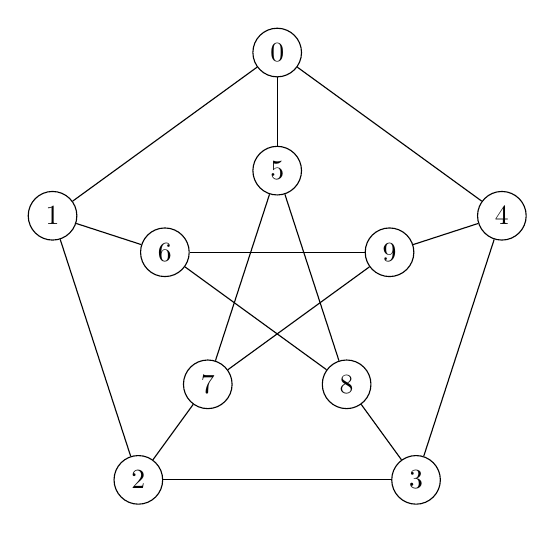
\begin{tikzpicture}
					% peterson graph labels;
					\def\outer {0,1,2,3,4};
					\def\inner {5,6,7,8,9};
					% radii
					\def\outerRadius {3};
					\def\innerRadius {1.5};
					% petersen graph outer layer
					\foreach \label [count=\index] in \outer
					{
						\node[draw, circle] (outer_\index) at (\index*72+18:\outerRadius) {\label};
					}
					% petersen graph inner layer
					\foreach \label [count=\index] in \inner
					{
						\node[draw, circle] (inner_\index) at (\index*72+18:\innerRadius) {\label};
					}
					% petersen graph edges
					\foreach \current in {1,...,5}
					{
						% outer
						\pgfmathtruncatemacro{\next}{mod(\current,5)+1};
						\draw (outer_\current) -- (outer_\next);
						% inner
						\pgfmathtruncatemacro{\next}{mod(\current+1,5)+1};
						\draw (inner_\current) -- (inner_\next);
						% crossing
						\draw (outer_\current) -- (inner_\current);
					}
				\end{tikzpicture}
			}
			\hspace*{\fill}
			\caption*{Graph 1}
		\end{subfigure}
		%
		\begin{subfigure}[b]{0.33\textwidth}
			\hspace*{\fill}
			\scalebox{0.6}
			{
				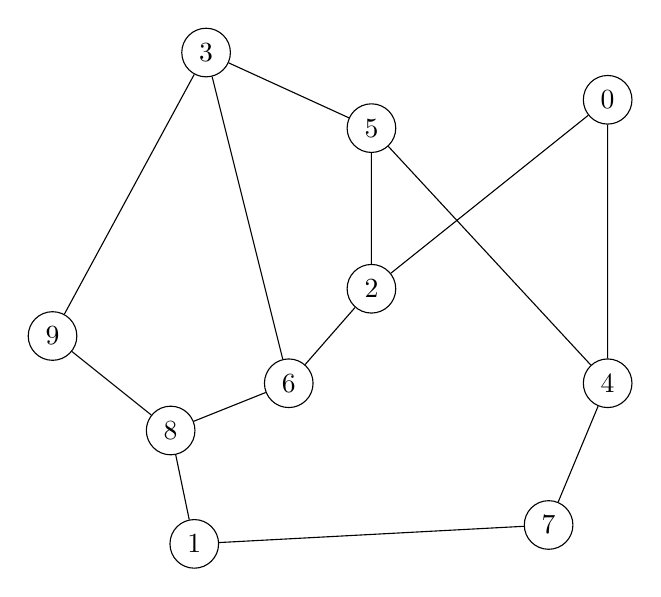
\begin{tikzpicture}
					% scale parameters
					\def\xscale {1.5};
					\def\yscale {1.2};
					% node labels
					\def\labels {9,8,1,6,3,5,2,0,4,7};
					% node xy coordinates
					\def\pos { (\xscale * 0   , 0     * \yscale)
							 , (\xscale * 1   , -1    * \yscale)
							 , (\xscale * 1.2 , -2.2  * \yscale)
							 , (\xscale * 2   , -0.5  * \yscale)
							 , (\xscale * 1.3 ,  3    * \yscale)
							 , (\xscale * 2.7 ,  2.2  * \yscale)
							 , (\xscale * 2.7 ,  0.5  * \yscale)
							 , (\xscale * 4.7 ,  2.5  * \yscale)
							 , (\xscale * 4.7 , -0.5  * \yscale)
							 , (\xscale * 4.2 , -2    * \yscale)
							 };
					% draw nodes and labels
					\foreach \coords [count=\index] in \pos
					{
						% node (v_\index) at \coords {\index};  % uncomment for debugging
						\node[draw, circle] (v_\index) at \coords {\phantom{0}};
					}
					\foreach \label [count=\index] in \labels
					{
						\node () at (v_\index) {\label};  % comment for debugging
					}
					% edges
					\draw  (v_2)  % path 1
						-- (v_3)
						-- (v_10)
						-- (v_9)
						-- (v_8)
						-- (v_7)
						-- (v_6)
						-- (v_9);
					\draw  (v_7)  % path 2
						-- (v_4)
						-- (v_2)
						-- (v_1)
						-- (v_5)
						-- (v_6);
					\draw  (v_5)
						-- (v_4);
				\end{tikzpicture}
			}
			\hspace*{\fill}
			\caption*{Graph 2}
		\end{subfigure}
		%
		\begin{subfigure}[b]{0.33\textwidth}
			\hspace*{\fill}
			\scalebox{0.6}
			{
				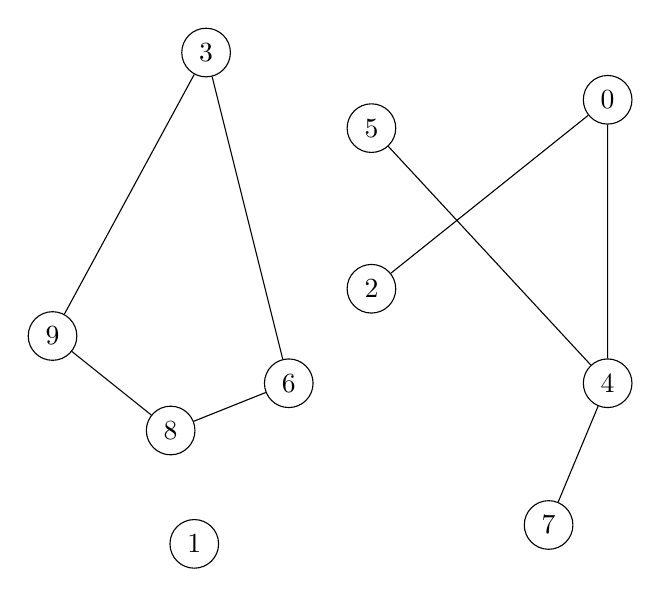
\begin{tikzpicture}
					% scale parameters
					\def\xscale {1.5};
					\def\yscale {1.2};
					% node labels
					\def\labels {9,8,1,6,3,5,2,0,4,7};
					% node xy coordinates
					\def\pos { (\xscale * 0   , 0     * \yscale)
							 , (\xscale * 1   , -1    * \yscale)
							 , (\xscale * 1.2 , -2.2  * \yscale)
							 , (\xscale * 2   , -0.5  * \yscale)
							 , (\xscale * 1.3 ,  3    * \yscale)
							 , (\xscale * 2.7 ,  2.2  * \yscale)
							 , (\xscale * 2.7 ,  0.5  * \yscale)
							 , (\xscale * 4.7 ,  2.5  * \yscale)
							 , (\xscale * 4.7 , -0.5  * \yscale)
							 , (\xscale * 4.2 , -2    * \yscale)
							 };
					% draw nodes and labels
					\foreach \coords [count=\index] in \pos
					{
						%\node (v_\index) at \coords {\index};  % uncomment for debugging
						\node[draw, circle] (v_\index) at \coords {\phantom{0}};
					}
					\foreach \label [count=\index] in \labels
					{
						\node () at (v_\index) {\label};  % comment for debugging
					}
					% edges
					\draw  (v_1)  % path 1
						-- (v_2)
						-- (v_4)
						-- (v_5)
						-- (v_1);
					\draw  (v_7)  % path 2
						-- (v_8)
						-- (v_9)
						-- (v_6);
					\draw  (v_10)
						-- (v_9);
				\end{tikzpicture}
			}
			\hspace*{\fill}
			\caption*{Graph 3}
		\end{subfigure}
		\caption{Graphen für Aufgabe 1. Graph 1 wird auch als \textit{Petersen-Graph} bezeichnet.}
		\label{ex1graph}
	\end{figure}
\end{center}


\begin{aufgabe}[Buchstabenlabyrinth \mittel]
	Algolina und ihre kleine Schwester spielen \emph{Buchstabenlabyrinth}.
	In diesem Spiel ist eine $N\times N$ Matrix gegeben, wo jeder Eintrag entweder A oder B ist. Zum Beispiel:
	\begin{center}
		\begin{tabular}{ccccc}
			\textbf{A} & A & \textbf{A} & \textbf{B} & \textbf{A}\\
			\textbf{B} & B & \textbf{B} & B & \textbf{B}\\
			\textbf{A} & \textbf{B} & \textbf{A} & A & \textbf{A}\\
			A & B & B & B & \textbf{B}\\
			A & A & A & A & \textbf{A}
		\end{tabular}
	\end{center}

	Die algorithmische Aufgabe ist es nun, einen kürzesten Pfad von oben links nach unten rechts zu finden.
	Die Knoten auf dem Pfad müssen dabei allerdings zwischen A und B alternieren, sprich die Knoten eines Pfades buchstabieren ABABABAB$\ldots$.
	Der Pfad darf in jedem Schritt immer nur horizontal oder vertikal gehen, diagonale Bewegungen sind also nicht erlaubt.
	Im Beispiel sind die Buchstaben des kürzesten Pfads fett geschrieben.

	Da die Schwestern sich nicht sicher sind, ob sie auch tatsächlich den kürzesten Weg gefunden haben, wollen sie ein Programm schreiben, das es für sie beantwortet.
	Entwirf einen Algorithmus, der für eine gegebene AB-Matrix die Länge eines kürzesten Weges findet.
	Implementiere den Algorithmus in einer Programmiersprache deiner Wahl.
\end{aufgabe}

\begin{aufgabe}[Tiefensuche mittels eines Stapels \bestehen]
	Erkläre, wie Tiefensuche ohne Rekursion mit einem Stapel implementiert werden kann.
\end{aufgabe}

\begin{aufgabe}[Wer nix weiß, sucht einen Kreis \bestehen]
	Entwirf einen Algorithmus, der feststellt, ob ein gegebener Graph einen Kreis enthält.
	Wie schnell ist dein Algorithmus?
\end{aufgabe}

\begin{aufgabe}[Anzahl kürzester Wege \bestehen]
	Entwirf einen Algorithmus, der für einen Graphen $G$ und zwei Knoten $s,t$ die Anzahl der kürzesten Pfade zwischen $s$ und $t$ ausgibt.
\end{aufgabe}

\begin{aufgabe}[Labyrinthe und Gittergraphen \schriftlich]
	Ein $k\times k$ Gittergraph ist ein Graph, in dem die Knoten, wie in einem Netz, in $k$ Zeilen mit jeweils $k$ Knoten angeordnet sind.
	Kanten dürfen sich hierbei nur zwischen Knoten befinden, die in horizontaler und vertikaler Richtung adjazent sind.
	Siehe Abbildung~\ref{ex6mazes}~(a).
	Löse die folgenden Teilaufgaben.
	\begin{enumerate}
		\item \bestehen Seien $n$ und $m$ die Anzahl der Knoten und Kanten in einem $k\times k$ Gittergraph.
		Drücke obere Schranken für $n$ und $m$ in asymptotischer Notation als Funktion von $k$ aus.
	\end{enumerate}
	Ein $k\times k$ Labyrinth ist eine quadratische Struktur, die aus $k$ Zeilen mit jeweils $k$ Zellen besteht.
	Jede Zelle wird durch vier Seiten begrenzt, und jede Seite ist entweder frei oder eine Wand.
	Ein Pfad im Labyrinth ist eine Sequenz $F$ von Zellen $f_1,\ldots, f_\ell$, sodass aufeinanderfolgende Zellen $f_i, f_{i+1}$ mit $1 \leq i < \ell$ horizontal oder vertikal adjazent sind und sich keine Wand zwischen ihnen befindet.
	Eine spezielle Zelle ist als Start gekennzeichnet und eine weitere als Ziel.\\
	Der Verein \enquote{Daten- und Gartenbau} bewertet ein Labyrinth als \textit{schön}, falls die folgenden Voraussetzungen eingehalten werden:
	\begin{itemize}
		\item Es gibt genau einen Weg vom Start zum Ziel.
		\item Es gibt einen Weg vom Start zu jeder anderen Zelle des Labyrinths.
		\item Es gibt keinen Weg, der im Kreis führt.
	\end{itemize}
	Ein Labyrinth wird als \textit{unschön} bewertet, wenn mindestens einer dieser Punkte verletzt wird.
	Siehe Abbildung~\ref{ex6mazes} (b)--(d).
	\begin{enumerate}
		\item[b)] \bestehen Beschreibe wie man ein $k\times k$ Labyrinth als $k\times k$ Gittergraph modelliert.
		\item[c)] \bestehen Zeichne Abbildung~\ref{ex6mazes} (b) als Gittergraph.
		\item[d)] \mittel Mit dem Aufschwung der Gärtnerei im letzten Jahr wurden nun so viele Labyrinthe eingereicht, dass der Verein es nun nicht mehr stemmen kann, jedes Labyrinth von Hand zu bewerten.
		Entwirf einen Algorithmus, der als Eingabe einen $k\times k$ Gittergraph erhält, der ein $k\times k$ Labyrinth modelliert, und prüft, ob das Labyrinth schön ist.
		Zeige die Korrektheit des Algorithmus\footnote{Beweis, dass die Ausgabe deines Algorithmus auf allen möglichen Eingaben richtig ist.} und gib eine Laufzeitanalyse an, in der die asymptotische Laufzeit als Funktion von $k$ beschreiben wird.
	\end{enumerate}
\end{aufgabe}
\begin{center}
	\begin{figure}[h]
		\begin{subfigure}[b]{0.24\textwidth}
			\hspace*{\fill}
			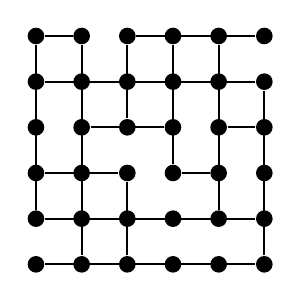
\begin{tikzpicture}
				\def\scale {0.58};
				% draw 6x6 node grid
				\foreach \x in {1,...,6}
				{
					\foreach \y in {1,...,6}
					{
						\node[fill=black, circle, inner sep=0pt, minimum size=6pt] (\x_\y) at (\scale * \x,\y * \scale) {};
					}
				}
				% horizontal edges
				\draw[thick] (1_1) -- (6_1);
				\draw[thick] (1_2) -- (6_2);
				\draw[thick] (1_3) -- (3_3);
				\draw[thick] (4_3) -- (5_3);
				\draw[thick] (2_4) -- (4_4);
				\draw[thick] (5_4) -- (6_4);
				\draw[thick] (1_5) -- (6_5);
				\draw[thick] (1_6) -- (2_6);
				\draw[thick] (3_6) -- (6_6);
				% vertical edges
				\draw[thick] (1_2) -- (1_6);
				\draw[thick] (2_1) -- (2_6);
				\draw[thick] (3_1) -- (3_3);
				\draw[thick] (3_4) -- (3_6);
				\draw[thick] (4_3) -- (4_6);
				\draw[thick] (5_2) -- (5_6);
				\draw[thick] (6_1) -- (6_5);
			\end{tikzpicture}	
			\hspace*{\fill}
			\caption{}
		\end{subfigure}
		\begin{subfigure}[b]{0.24\textwidth}
			\hspace*{\fill}
			\scalebox{0.5}
			{
				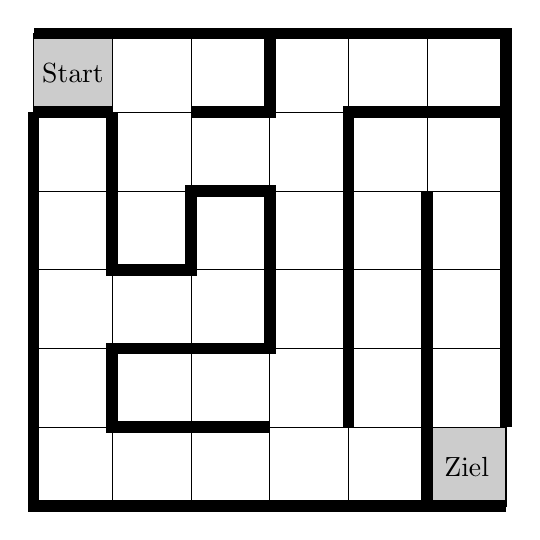
\begin{tikzpicture}
					% 6x6 grid
					\draw (0,0) grid (6,6);
					% target label backdrops
					\draw[fill=black!20] (5,1) rectangle (6,0);
					\draw[fill=black!20] (0,6) rectangle (1,5);
					% target labels
					\node () at (5.5,0.5) {Ziel};
					\node () at (0.5,5.5) {Start};                
	
					% ####################################
					%
					% toggle options
					% option (b): wall south to start
					\draw[line width=1.5mm] (0,5) -- (1,5);
					%
					% option (c): red filled rectangle and additional wall
					% \fill[red] (4,1) rectangle (5,0); \draw[line width=1.5mm] (4,0) -- (4,1);
					%
					% option (d) dashed red line
					% \draw[line width=1mm, dashed, red] (0.5,5.5) -- (0.5,0.5) -- (3.5,0.5) -- (3.5,4.5) -- (1.5,4.5) -- (1.5,5.5) -- (0.5,5.5);
					%
					% ####################################
	
					% walls
					\draw[line width=1.5mm]
								 (6,0)
							  -- (0,0)
							  -- (0,5);
					\draw[line width=1.5mm]
								 (1,5)
							  -- (1,3)
							  -- (2,3)
							  -- (2,4)
							  -- (3,4)
							  -- (3,2)
							  -- (1,2)
							  -- (1,1)
							  -- (3,1);
					\draw[line width=1.5mm]
								 (5,0)
							  -- (5,4);
					\draw[line width=1.5mm]
								 (4,1)
							  -- (4,5)
							  -- (6,5)
							  -- (6,1);
					\draw[line width=1.5mm]
								 (6,5)
							  -- (6,6)
							  -- (0,6);
					\draw[line width=1.5mm]
								 (3,6)
							  -- (3,5)
							  -- (2,5);
				\end{tikzpicture}    
			}	
			\hspace*{\fill}
			\caption{}
		\end{subfigure}
		\begin{subfigure}[b]{0.24\textwidth}
			\hspace*{\fill}
			\scalebox{0.5}
			{
				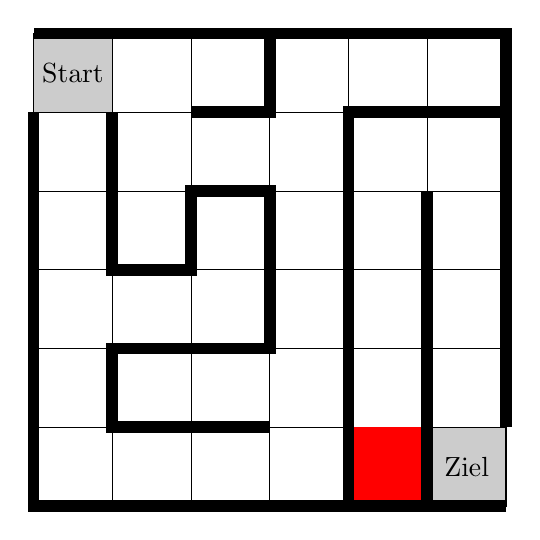
\begin{tikzpicture}
					% 6x6 grid
					\draw (0,0) grid (6,6);
					% target label backdrops
					\draw[fill=black!20] (5,1) rectangle (6,0);
					\draw[fill=black!20] (0,6) rectangle (1,5);
					% target labels
					\node () at (5.5,0.5) {Ziel};
					\node () at (0.5,5.5) {Start};                
	
					% ####################################
					%
					% toggle options
					% option (b): wall south to start
					%\draw[line width=1.5mm] (0,5) -- (1,5);
					%
					% option (c): red filled rectangle and additional wall
					\fill[red] (4,1) rectangle (5,0); \draw[line width=1.5mm] (4,0) -- (4,1);
					%
					% option (d) dashed red line
					% \draw[line width=1mm, dashed, red] (0.5,5.5) -- (0.5,0.5) -- (3.5,0.5) -- (3.5,4.5) -- (1.5,4.5) -- (1.5,5.5) -- (0.5,5.5);
					%
					% ####################################
	
					% walls
					\draw[line width=1.5mm]
								 (6,0)
							  -- (0,0)
							  -- (0,5);
					\draw[line width=1.5mm]
								 (1,5)
							  -- (1,3)
							  -- (2,3)
							  -- (2,4)
							  -- (3,4)
							  -- (3,2)
							  -- (1,2)
							  -- (1,1)
							  -- (3,1);
					\draw[line width=1.5mm]
								 (5,0)
							  -- (5,4);
					\draw[line width=1.5mm]
								 (4,1)
							  -- (4,5)
							  -- (6,5)
							  -- (6,1);
					\draw[line width=1.5mm]
								 (6,5)
							  -- (6,6)
							  -- (0,6);
					\draw[line width=1.5mm]
								 (3,6)
							  -- (3,5)
							  -- (2,5);
				\end{tikzpicture}    
			}	
			\hspace*{\fill}
			\caption{}
		\end{subfigure}
		\begin{subfigure}[b]{0.24\textwidth}
			\hspace*{\fill}
			\scalebox{0.5}
			{
				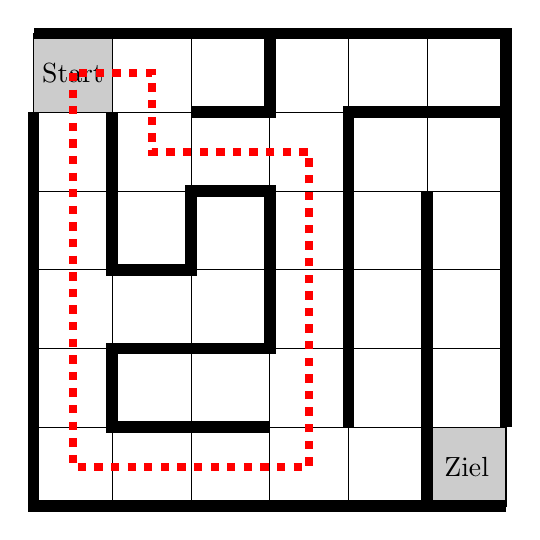
\begin{tikzpicture}
					% 6x6 grid
					\draw (0,0) grid (6,6);
					% target label backdrops
					\draw[fill=black!20] (5,1) rectangle (6,0);
					\draw[fill=black!20] (0,6) rectangle (1,5);
					% target labels
					\node () at (5.5,0.5) {Ziel};
					\node () at (0.5,5.5) {Start};                
	
					% ####################################
					%
					% toggle options
					% option (b): wall south to start
					%\draw[line width=1.5mm] (0,5) -- (1,5);
					%
					% option (c): red filled rectangle and additional wall
					% \fill[red] (4,1) rectangle (5,0); \draw[line width=1.5mm] (4,0) -- (4,1);
					%
					% option (d) dashed red line
					\draw[line width=1mm, dashed, red] (0.5,5.5) -- (0.5,0.5) -- (3.5,0.5) -- (3.5,4.5) -- (1.5,4.5) -- (1.5,5.5) -- (0.5,5.5);
					%
					% ####################################
	
					% walls
					\draw[line width=1.5mm]
								 (6,0)
							  -- (0,0)
							  -- (0,5);
					\draw[line width=1.5mm]
								 (1,5)
							  -- (1,3)
							  -- (2,3)
							  -- (2,4)
							  -- (3,4)
							  -- (3,2)
							  -- (1,2)
							  -- (1,1)
							  -- (3,1);
					\draw[line width=1.5mm]
								 (5,0)
							  -- (5,4);
					\draw[line width=1.5mm]
								 (4,1)
							  -- (4,5)
							  -- (6,5)
							  -- (6,1);
					\draw[line width=1.5mm]
								 (6,5)
							  -- (6,6)
							  -- (0,6);
					\draw[line width=1.5mm]
								 (3,6)
							  -- (3,5)
							  -- (2,5);
				\end{tikzpicture}    
			}	
			\hspace*{\fill}
			\caption{}
		\end{subfigure}
		\caption{\label{ex6mazes}(a) ein $6\times6$ Gittergraph. (b), (c) und (d) sind $6\times6$ Labyrinthe. (b) ist schön, (c) und (d) sind unschön. In (c) ist das Ende nicht erreichbar und (d) enthält einen Weg der im Kreis führt.}
	\end{figure}
\end{center}

\begin{aufgabe}[Eulerkreis und Eulerpfad]
	Sei $G$ ein zusammenhängender Graph mit $n$ Knoten und $m$ Kanten.
	Ein Eulerpfad in $G$ ist ein Pfad, der alle Kanten genau ein mal enthält.
	Ein Eulerkreis ist ein Eulerpfad, der in demselben Knoten beginnt und endet.
	Löse die folgenden Teilaufgaben.
	\begin{enumerate}
		\item \note %(\hard)
    Beweise, dass $G$ einen Eulerkreis genau dann enthält, wenn alle Knoten einen geraden Knotengrad haben.
		\item \note %(\hard)
    Beweise, dass $G$ einen Eulerpfad genau dann enthält, wenn 0 oder 2 Knoten einen ungeraden Knotengrad haben.
		\item \bestehen Welche dieser Zeichnungen können gezeichnet werden ohne den Stift abzusetzen?
		Kannst du den Stift am selben Punkt auf- und absetzen?
	\end{enumerate}
	\begin{center}
		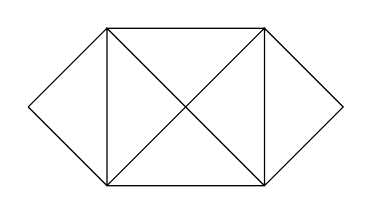
\begin{tikzpicture}
			% graph 1 has an euler tour :D
			% no dont tell them :(
			\draw (0,0) -- (1,-1) -- (2,0) -- (3,-1) -- (4,0) -- (3,1) -- (3,-1) -- (1,-1) -- (1,1) -- (2,0) -- (3,1) -- (1,1) -- (0,0);
		\end{tikzpicture}
		%
		\hspace{1.5cm}
		%
		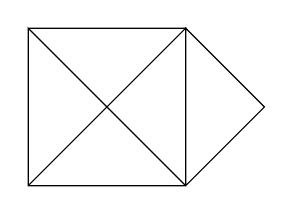
\begin{tikzpicture}
			% graph 2 has an euler tour :D
			\draw (1,-1) -- (2,0) -- (3,-1) -- (4,0) -- (3,1) -- (3,-1) -- (1,-1) -- (1,1) -- (2,0) -- (3,1) -- (1,1);
		\end{tikzpicture}
		%
		\hspace{1.5cm}
		%
		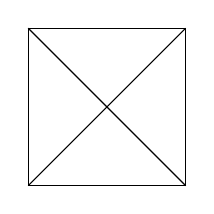
\begin{tikzpicture}
			% graph 3 does not :D
			\draw (1,-1) -- (3,-1) -- (3,1) -- (1,1) -- (1,-1);
			\draw (1,-1) -- (3,1);
			\draw (1,1) -- (3,-1);
		\end{tikzpicture}
	\end{center}
	\begin{enumerate}[resume]
		\item \bestehen Entwirf einen Algorithmus, der in Zeit $O(n+m)$ ermittelt, ob $G$ einen Eulerkreis enthält.
		\item \note %(\hard)
    Entwirf einen Algorithmus, der in Zeit $O(n+m)$ einen Eulerkreis ausgibt, falls $G$ einen enthält.
	\end{enumerate}	
\end{aufgabe}


\begin{aufgabe}[Durchmesser von Bäumen]
	Sei $T$ ein binärer Baum mit $n$ Knoten.
	Der \textit{Durchmesser von $T$} ist die Länge des längsten kürzesten Weges zwischen Knotenpaaren aus $T$.\footnote{Sei $dist_G(u,v)$ die Länge des kürzesten Weges von Knoten $u$ nach Knoten $v$ im Graph $G$, dann ist der Durchmesser $\max_{u,v\in G}( dist_G(u,v) )$.}
	\begin{enumerate}
		\item \mittel Entwirf einen Algorithmus, der den Durchmesser von $T$ in Zeit $O(n^2)$ ermittelt.
		\item \note (\veryhard) Entwirf einen Algorithmus, der den Durchmesser von $T$ in Zeit $O(n)$ ermittelt.
	\end{enumerate}
\end{aufgabe}

\begin{aufgabe}[3-Farben Algorithmus]
  \textit{\footnotesize For an English version of this exercise, see [\href{https://jeffe.cs.illinois.edu/teaching/algorithms/book/Algorithms-JeffE.pdf}{Erickson}, page 210]}.\\
  Eine Klasse von Suchalgorithmen auf Graphen, die Breitensuche und Tiefensuche verallgemeinern, wurde 1975 von Edsger Dijkstra, Leslie Lamport, Alain Martin, Carel Scholten und Elisabeth Steffens beschrieben. Die Autor:innen haben diese Algorithmen untersucht, um damit einen automatischen \emph{garbage collector} zu entwerfen (siehe \href{https://de.wikipedia.org/wiki/Garbage_Collection}{wikipedia}).
  Anstatt markierte und unmarkierte Knoten zu verwalten, verwaltet ihr Algorithmus eine Farbe für jeden Knoten, entweder weiß, grau oder schwarz.
  Im Folgenden stellen wir uns einen als Adjazenzliste gegebenen, ungerichteten Graphen $G$ vor.
  
  \begin{tabular}{p{0.44\textwidth}p{0.49\textwidth}}
  \mbox{}\begin{algorithmic}
      \Procedure{ThreeColorSearch}{s}
      \State{färbe alle Knoten weiß}
      \State{färbe $s$ grau}
      \While{mindestens ein Knoten ist grau}
          \State{\Call{ThreeColorStep}{}}
      \EndWhile{}
      \EndProcedure{}
  \end{algorithmic}
  &
  \mbox{}\begin{algorithmic}
      \Procedure{ThreeColorStep}{}
      \State{$v\gets$ irgendein grauer Knoten}
      \If{$v$ hat keine weißen Nachbarn}
          \State{färbe $v$ schwarz}
      \Else{}
          \State{$w\gets$irgendein weißer Nachbar von $v$}
          \State{$w.\pi\gets v$} \Comment{$v$ ist der Elternknoten von $w$.}
          \State{färbe $w$ grau}
      \EndIf{}
      \EndProcedure{}
  \end{algorithmic}
  \end{tabular}
  
  \begin{enumerate}
      \item\label{Farbinvariante} \bestehen Beweise, dass \textsc{ThreeColorSearch} zu jedem Zeitpunkt die folgende Invariante erhält: Kein schwarzer Knoten ist zu einem weißen Knoten benachbart. \emph{(Hinweis: Das sollte einfach sein.)}
      \item \mittel Beweise Folgendes: Wenn \textsc{ThreeColorSearch}$(s)$ terminiert, dann sind alle von $s$ erreichbaren Knoten schwarz, alle nicht von $s$ erreichbaren Knoten weiß, und die zu den Eltern zeigenden Kanten $(v, v.\pi)$ definieren einen Baum, der alle Knoten der Zusammenhangskomponente von $s$ aufspannt.
      \emph{Hinweis: Wenn man den Algorithmus mit DFS/BFS vergleicht, kann man sich intuitiv vorstellen, dass die schwarzen Knoten \enquote{markiert} sind und die grauen Knoten \enquote{auf dem Stapel/in der Warteschlange}. Ein Unterschied ist, dass \textsc{ThreeColorStep} nicht im selben Aufruf \emph{alle} Kanten abarbeiten muss, die aus einem Knoten $v$ rausgehen.}
      \item \mittel Die folgende Variante von \textsc{ThreeColorSearch} verwaltet die grauen Knoten auf einem Stapel.
      Beweise, dass diese Variante äquivalent zu DFS ist, das heißt, die Knoten werden in genau derselben Reihenfolge entdeckt und die Elternbeziehungen sind identisch.
      \emph{Hinweis: Die Reihenfolge der letzten zwei Zeilen von \textsc{ThreeColorStackStep} ist wichtig!}
  
      \begin{tabular}{p{0.44\textwidth}p{0.49\textwidth}}
          \mbox{}\begin{algorithmic}
              \Procedure{ThreeColorStackSearch}{$s$}
              \State{färbe alle Knoten weiß}
              \State{färbe $s$ grau}
              \State{\fett{lege $s$ auf den Stapel}}
              \While{mindestens ein Knoten ist grau}
                  \State{\Call{ThreeColorStackStep}{}}
              \EndWhile{}
              \EndProcedure{}
          \end{algorithmic}
          &
          \mbox{}\begin{algorithmic}
              \Procedure{ThreeColorStackStep}{}
              \State{\fett{nimm $v$ vom Stapel}}
              \If{$v$ hat keine weißen Nachbarn}
                  \State{färbe $v$ schwarz}
              \Else{}
                  \State{$w\gets$irgendein weißer Nachbar von $v$}
                  \State{$w.\pi\gets v$}
                  \State{färbe $w$ grau}
                  \State{\fett{lege $v$ auf den Stapel}}
                  \State{\fett{lege $w$ auf den Stapel}}
              \EndIf{}
              \EndProcedure{}
          \end{algorithmic}
          \end{tabular}
  
      \item\label{notBFS} \mittel Die folgende Variante von \textsc{ThreeColorSearch} verwaltet die grauen Knoten in einer Warteschlange.
      Beweise, dass diese Variante \emph{\textbf{nicht}} äquivalent zu BFS ist.
      \emph{Hinweis: Die Reihenfolge der letzten zwei Zeilen von \textsc{ThreeColorQueueStep} ist nicht wichtig!}
      
          \begin{tabular}{p{0.44\textwidth}p{0.49\textwidth}}
              \mbox{}\begin{algorithmic}
                  \Procedure{ThreeColorQueueSearch}{$s$}
                  \State{färbe alle Knoten weiß}
                  \State{färbe $s$ grau}
                  \State{\fett{schiebe $s$ in die Warteschlange}}
                  \While{mindestens ein Knoten ist grau}
                      \State{\Call{ThreeColorQueueStep}{}}
                  \EndWhile{}
                  \EndProcedure{}
              \end{algorithmic}
              &
              \mbox{}\begin{algorithmic}
                  \Procedure{ThreeColorQueueStep}{}
                  \State{\fett{ziehe $v$ aus der Warteschlange}}
                  \If{$v$ hat keine weißen Nachbarn}
                      \State{färbe $v$ schwarz}
                  \Else{}
                      \State{$w\gets$irgendein weißer Nachbar von $v$}
                      \State{$w.\pi\gets v$}
                      \State{färbe $w$ grau}
                      \State{\fett{schiebe $v$ in die Warteschlange}}
                      \State{\fett{schiebe $w$ in die Warteschlange}}
                  \EndIf{}
                  \EndProcedure{}
              \end{algorithmic}
              \end{tabular}
  
      \item \note (\veryhard) Hier sei $G$ ein gerichteter Graph. Wir nehmen nun an, dass ein zweiter Prozess Kanten zu $G$ hinzufügt, während \textsc{ThreeColorSearch} noch läuft. Diese neuen Kanten könnten die Farbinvariante zerstören, die in Teil~\ref{Farbinvariante} beschrieben ist. Daher könnte es jetzt sein, dass \textsc{ThreeColorSearch} nicht mehr korrekt ist. Das heißt, es könnte sein, dass der Algorithmus zwar terminiert, aber es trotzdem noch Knoten gibt, die von $s$ erreichbar sind und weiß sind. Wenn wir einen \emph{garbage collector} implementieren wollen, wäre das fatal, denn hier würden wir \enquote{weiß} mit \enquote{unerreichbar und daher löschbar} gleichsetzen wollen.
      
      Wenn der andere Prozess auf die Farbinvariante Rücksicht nimmt und diese explizit wiederherstellt, wann immer sie verletzt würde, dann können wir den \textsc{ThreeColorSearch} Algorithmus trotzdem sicher verwenden. Das möchten wir jetzt zeigen. Um die zwei parallelen Algorithmen zu modellieren, verwenden wir die \emph{either/or} Syntax in \textsc{GarbageCollect}; wie bei \emph{if/then/else} verzweigt das Programm hier, aber welcher Zweig verfolgt wird, wird nicht vom Programm selbst entschieden, sondern vom Betriebssystem.\footnote{Das ist eine dramatische Vereinfachung, sowohl von paralleler Programmierung als auch von \emph{garbage collection}. Mehrfädige Programmiersprachen wie Lua und Go benutzen einen viel komplexeren \emph{mark and sweep} Algorithmus als \emph{garbage collector}. Mathematisch wichtig für \emph{either/or} ist, dass das Betriebssystem zwar nicht garantiert, wie oft hintereinander und in welcher Reihenfolge die zwei Programmzweige gewählt werden. Aber jeder Zweig wird immer wieder \emph{irgendwann} gewählt, das heißt, nach endlicher Zeit. --- Das Betriebsystem darf also \emph{\textbf{nicht}} für immer den einen Zweig wählen und den anderen \enquote{vergessen}.}
  
      \begin{tabular}{p{0.44\textwidth}p{0.49\textwidth}}
          \mbox{}\begin{algorithmic}
              \Procedure{GarbageCollect}{$s$}
              \State{färbe alle Knoten weiß}
              \State{färbe $s$ grau}
              \While{mindestens ein Knoten ist grau}
                  \State{\fett{either}}
                      \State{\quad\Call{CollectStep}{}}
                  \State{\fett{or}}
                      \State{\quad\fett{\Call{Mutate}{}}}
              \EndWhile{}
              \EndProcedure{}
          \end{algorithmic}
          &
          \mbox{}\begin{algorithmic}
              \Procedure{CollectStep}{}
              \State{$v\gets$ irgendein grauer Knoten}
              \If{$v$ hat keine weißen Nachbarn}
                  \State{färbe $v$ schwarz}
              \Else{}
                  \State{$w\gets$irgendein weißer Nachbar von $v$}
                  \State{färbe $w$ grau}
              \EndIf{}
              \EndProcedure{}
          \end{algorithmic}\\
          \mbox{}\begin{algorithmic}
              \Procedure{Mutate}{}
              \State{$u\gets$ irgendein Knoten}
              \State{$w\gets$ irgendein Knoten}
              \If{$(u,w)$ ist keine Kante}
                  \State{füge $(u,w)$ als Kante hinzu}
                  \If{$u$ ist schwarz und $w$ ist weiß}
                  \State{färbe $u$ grau}
                  \EndIf{}
                  \If{$u$ ist weiß und $w$ ist schwarz}
                  \State{färbe $w$ grau}
                  \EndIf{}
              \EndIf{}
              \EndProcedure{}
          \end{algorithmic}
          \end{tabular}
  
          Beweise, dass \textsc{GarbageCollect} irgendwann terminiert, und dass dann jeder von $s$ erreichbare Knoten schwarz gefärbt ist und jeder von $s$ nicht erreichbare Knoten weiß gefärbt ist.
      \item \note (\veryhard) Hier sei $G$ wieder ein gerichteter Graph. Anstatt schwarze Knoten grau zu färben, soll \textsc{Mutate} jetzt die Farbinvariante aufrechterhalten, indem manche \emph{weißen} Knoten grau gefärbt werden:
      \begin{algorithmic}
          \Procedure{Mutate}{}
          \State{$u\gets$ irgendein Knoten}
          \State{$w\gets$ irgendein Knoten}
          \If{$(u,w)$ ist keine Kante}
              \State{füge $(u,w)$ als Kante hinzu}
              \If{$u$ ist schwarz und $w$ ist weiß}
              \State{\fett{färbe $w$ grau}}
              \EndIf{}
              \If{$u$ ist weiß und $w$ ist schwarz}
              \State{\fett{färbe $u$ grau}}
              \EndIf{}
          \EndIf{}
          \EndProcedure{}
      \end{algorithmic}
      Beweise, dass \textsc{GarbageCollect} irgendwann terminiert, und dass dann $s$ schwarz gefärbt ist, jeder von einem schwarzen Knoten erreichbare Knoten wiederum schwarz ist, und jeder nicht von einem schwarzen Knoten erreichbare Knoten weiß ist.
  \end{enumerate}
  
\end{aufgabe}

\end{document}
